\section{Exploration in \awa}
I implemented two exploration techniques within the framework of \awa. The general idea is that for each node expansion, there is some probability $\epsilon$ that instead of expanding the best node according to the weighted evaluation function $f(n)$, some other node, in a knowledge-free way, is chosen from the open list for expansion. The two proposed techniques are \egreedy and \ebgreedy.

\subsection{\eawa}
\eawa employs the \egreedy exploration and works much the same as $\epsilon$-GBFS (in an anytime context). With this technique, with probability $\epsilon$, a node is chosen uniformly at random from the open list.

Using \egreedy in \awa simply means potentially selecting an exploratory node during the node selection phase on Line 5 in Algorithm \ref{alg:awa}. Replacing Line 5 with the procedure outlined in Algorithm \ref{alg:eawa} gives \eawa, where \texttt{randomSample} samples uniformly at random from the open list, and \texttt{randrange} samples uniformly at random from the given range.

\begin{algorithm}
\caption{$\epsilon-$AWA$^*$ node selection}\label{alg:eawa}
\begin{algorithmic}
\State $y \gets $ randrange(0,1)
\If{$y \leq \epsilon$}
    \State\Return randomSample($OPEN$)
\Else{}
    \State\Return $\arg \min_{x \in OPEN} f'(x)$
\EndIf
\end{algorithmic}
\end{algorithm}

\subsection{\ebawa}
\ebawa employs \ebgreedy sampling, which is a bit more involved than \egreedy and is meant to address some of the shortcomings of \egreedy sampling. Xie's Type-Based sampling, along with its use in WA$^*$ by Cohen \textit{et al.}, serves as the inspiration for the \ebgreedy sampling devised for \ebawa--where the aim is to achieve a better spread over the state space during sampling.

Simply put, \ebgreedy samples from the open list non-uniformly. It is assumed that the open list is stored as a minimum heap; then the sampling is done in two steps: first sample a row from the heap non-uniformly, second sample a node uniformly from that row. The non-uniform sampling of a row is done according to a beta distribution, $B(\alpha, \beta)$, hence \ebgreedy. Looking at Figure \ref{fig:beta}, sampling a row can be thought of as evenly spacing the rows between 0 and 1 along the x-axis and then sampling one according to the probability density above it. The intuition behind this is that, while heaps don't make strong guarantees about the order of nodes, they do guarantee that a parent is larger than both its children. This means that, in general, sampling from higher rows will yield smaller f-cost nodes than sampling from lower rows. And so, if you bias your row sampling to middling or lower rows you should expect to see a better spread across the state space. Furthermore, I think it's a fair assumption that those nodes with smaller f-costs are likely to be expanded sooner in the usual way (i.e. by the selection done on Line 5 in Algorithm \ref{alg:awa}) regardless of plateaus, and so exploration should focus on those nodes that aren't close to conventional expansion. This sampling technique also benefits from being quite simple to implement.

\begin{algorithm}
\caption{\ebawa node selection}\label{alg:abawa}
\begin{algorithmic}
\Require $\gamma \gets beta(\alpha, \beta)$
\State $y \gets $ randrange(0,1)
\If{$y \leq epsilon$}
    \State $row \gets $ sampleRow($OPEN$, $\gamma$)
    \State $start \gets 2^{row}-1$
    \State $end \gets 2 \cdot start$
    \State \Return randomSample($OPEN[start:end]$)
\Else{}
    \State \Return $\arg \min_{x \in OPEN} f'(x)$
\EndIf
\end{algorithmic}
\end{algorithm}

Much like in \eawa, the two-step sampling of \ebgreedy is employed in \ebawa at each expansion with probability $\epsilon$. The procedure outlined in Algorithm \ref{alg:abawa} can be invoked instead of Line 5 in Algorithm \ref{alg:awa} to get \ebawa.

\noindent
\begin{figure}
    \begin{center}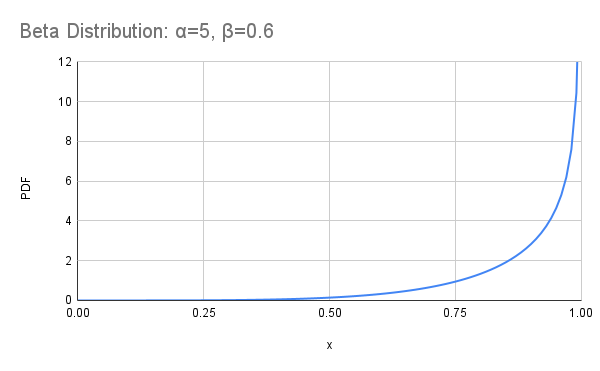
\includegraphics[scale=0.35]{media/beta.png}\end{center}
    \caption{Beta Distribution used in \ebawa}\label{fig:beta}
\end{figure}